\chapter{Introduction}

This User's Guide contains a description of the software, its capabilities and instructions for installing Lattice Microbes, the software described in the following publications: \cite{Roberts2009lts,Roberts2013lmh,Hallock2014sor}. This guide is very much a work in progress and will continue to be expanded. At present, it should contain enough information to get you started using the Lattice Microbes software.

%%%%%%%%%%%%%%%
% Section: Lattice Microbes %
%%%%%%%%%%%%%%%
\section{Lattice Microbes}
Studying cellular processes, which show inherently noisy non-deterministic behavior, with single molecule resolution on timescales of biological relevance such as the lifetime of a cell, requires considerable computational effort.  Lattice Microbes \cite{Roberts2009lts,Roberts2013lmh} is software developed to sample realizations of the spatially homogenous and heterogeneous stochastic Master equations, with thousands of reactions among hundreds of molecular species.  The software uses graphics processing units (GPUs) to exploit the natural parallelism afforded by the Master equations to access timescales orders-of-magnitude larger than other particle-- and grid--based software for sampling stochastic cellular processes as seen in Figure \ref{fig:timings}. While Lattice Microbes was originally designed for simulating single \emph{E. coli} cells on one GPU, the desire to simulate cellular consortia and larger species like yeast, drove the development of a new version of Lattice Microbes that utilizes multiple GPUs to share the work \cite{Hallock2014sor}. In addition to larger simulations, multiple GPUs allow small simulations to be completed more quickly.

\begin{figure}[h!]
  \centering
      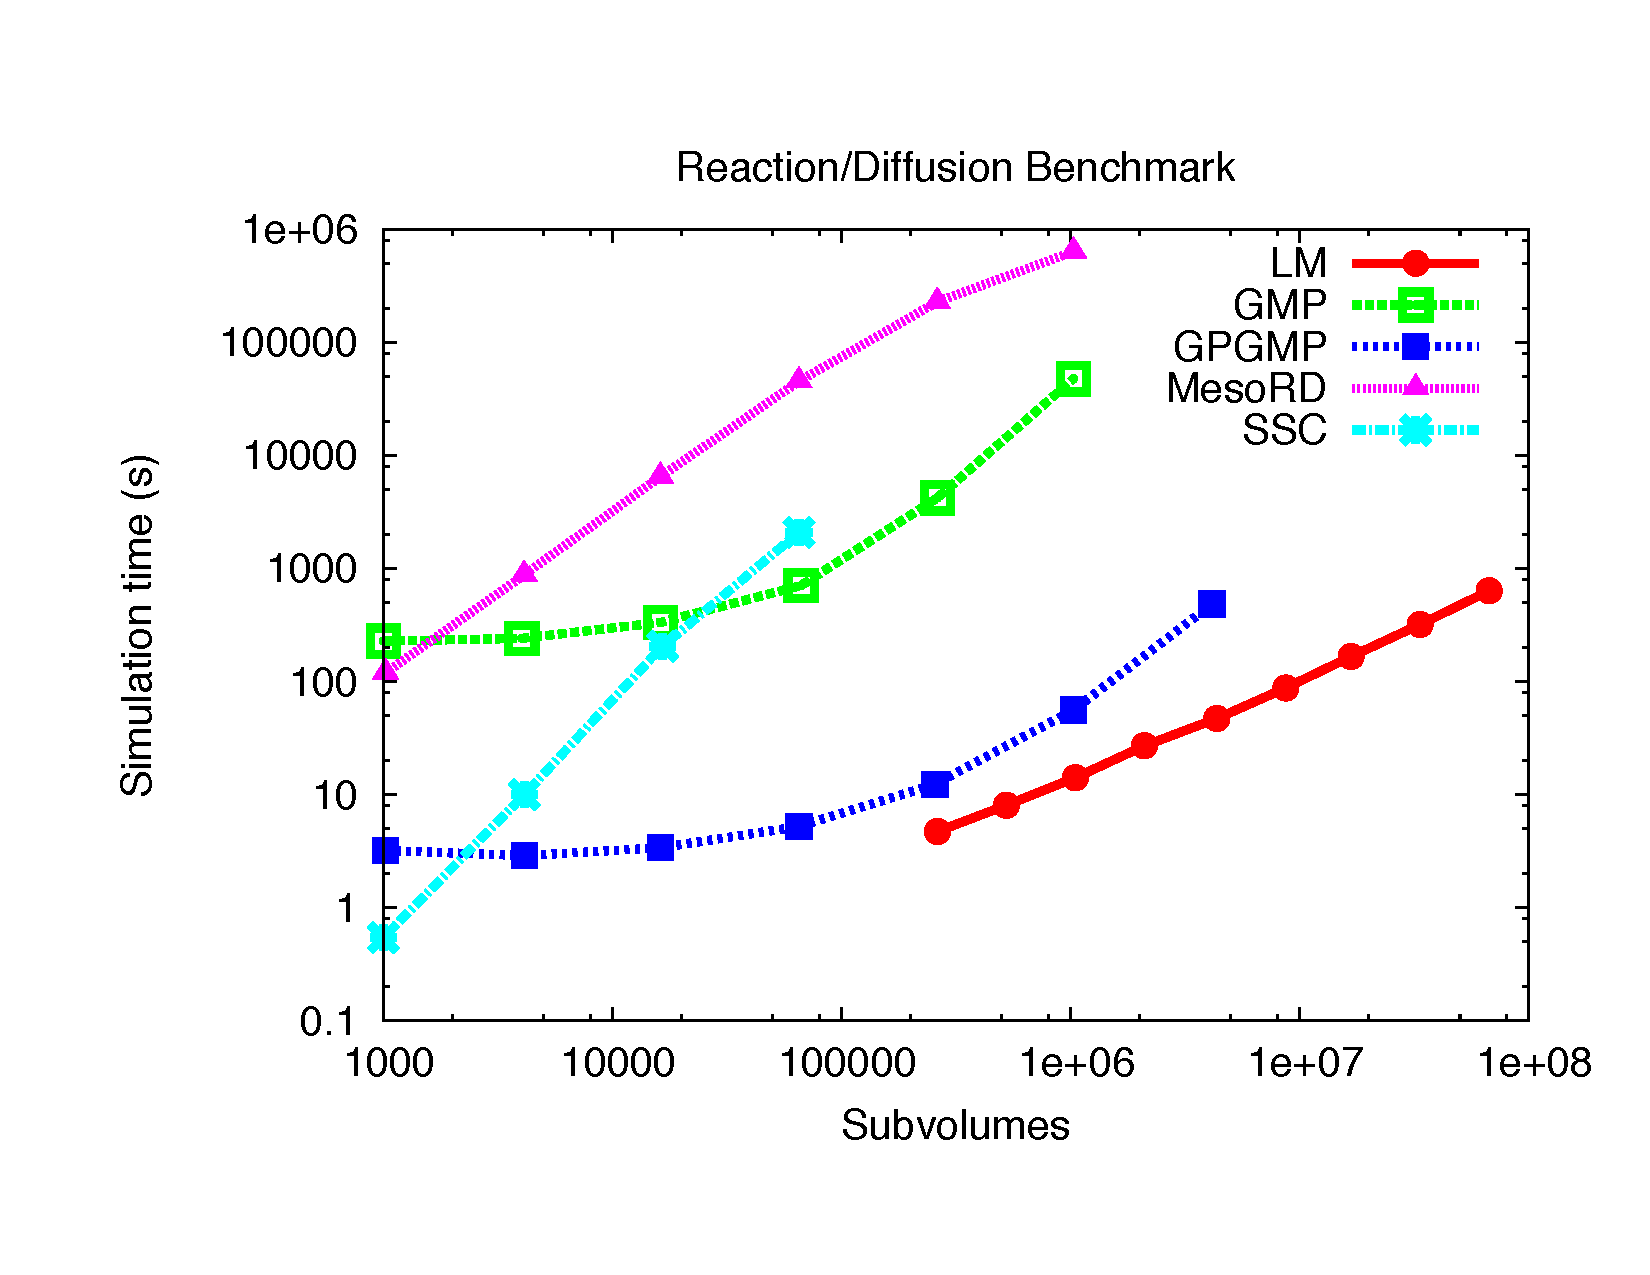
\includegraphics[width=0.75\textwidth]{Figures/SoftwareBenchmark.pdf}
  \caption{Comparison (lower is better) of simulation time to completion with Lattice Microbes  to other grid-based stochastic software for a simulation of spatially resolved reversible bimolecular reaction with 100K particles at different system volumes.  Data for other simulation codes from the paper: \cite{Vigelius2010ard}. Key: LM - ``Lattice Microbes Multi-particle diffusion RDME",  GMP - ``Gillespie Multi-Particle", GPGMP - ``GPU Gillespie Multi-Particle", MesoRD - ``MesoRD", SSC - ``Stochastic Simulation Compiler".} \label{fig:timings}
\end{figure}


%%%%%%%%%%
% Section: PyLM %
%%%%%%%%%%
\section{pyLM}
pyLM is a Problem Solving Environment (PSE) for biological simulations \cite{Peterson2013aps}.  Written in Python, it wraps and extends Lattice Microbes.  The PSE is comprised of a base set of functionality to set up, monitor and modify simulations, as well as a set of standard post--processing routines that interface to other Python packages, including NumPy, SciPy, H5py, and iGraph to name a few.  \\

\begin{figure}[h!]
  \centering
      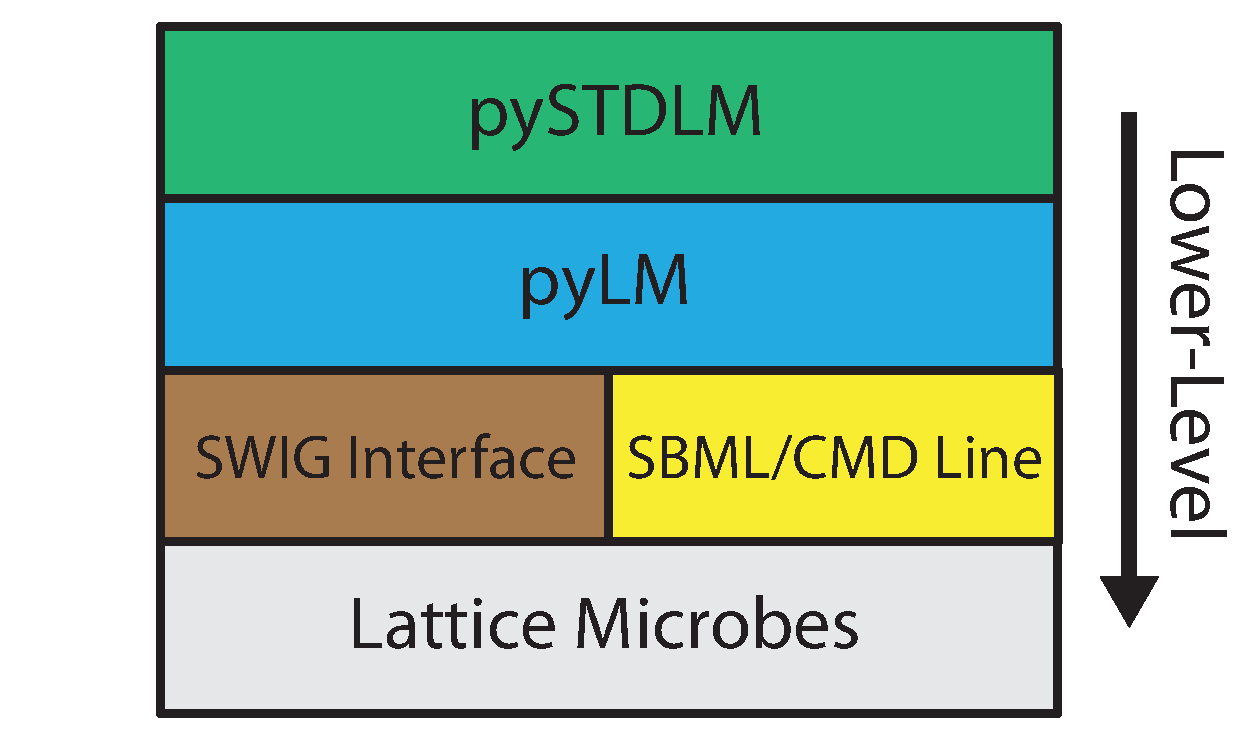
\includegraphics[width=0.7\textwidth]{Figures/Schematic.pdf}
  \caption{A schematic of the pyLM and the Lattice Microbes software.} \label{fig:pyschematic}
\end{figure}

The PSE is shown schematically in Figure \ref{fig:pyschematic}.  It sits on top of a SWIG interface that allows the C++ code to be accessible from the Python terminal.  Using pyLM allows the user to set up, run and post--process simulations all within a single script.  A general workflow for using LM is shown in Figure \ref{fig:workflow}.  For tutorials on using pyLM please see the ``Instruction Guide" and for in--depth description of all pyLM functionality please see the documentation ``Reference Guide" available on the website.

\begin{figure}[h!]
  \centering
      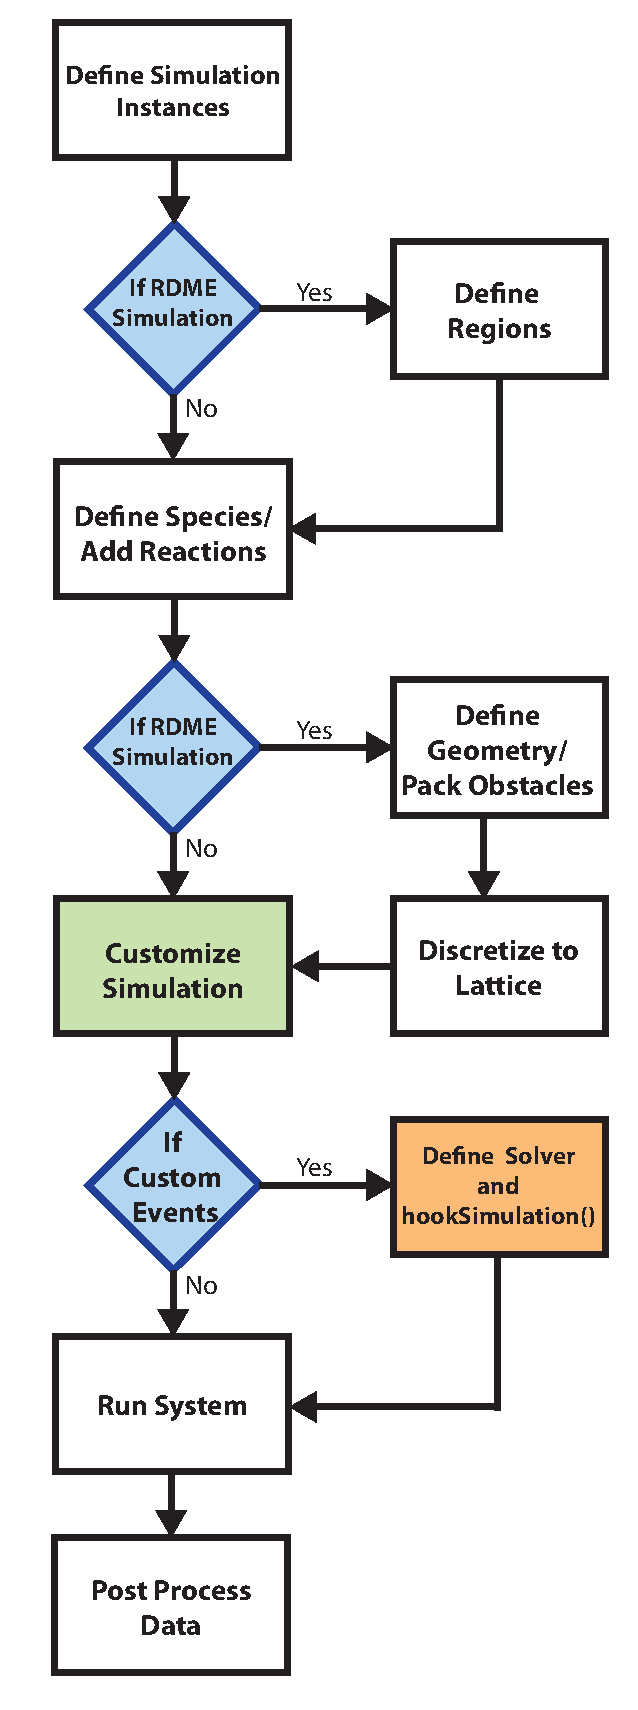
\includegraphics[width=0.5\textwidth]{Figures/Workflow.pdf}
  \caption{The workflow of the pyLM PSE.} \label{fig:workflow}
\end{figure}
